

\tikzset{every picture/.style={line width=0.75pt}} %set default line width to 0.75pt        

\begin{tikzpicture}[x=0.75pt,y=0.75pt,yscale=-0.89,xscale=0.89]
%uncomment if require: \path (0,173); %set diagram left start at 0, and has height of 173

%Image [id:dp08550642952575427] 
\draw (165.05,80.66) node  {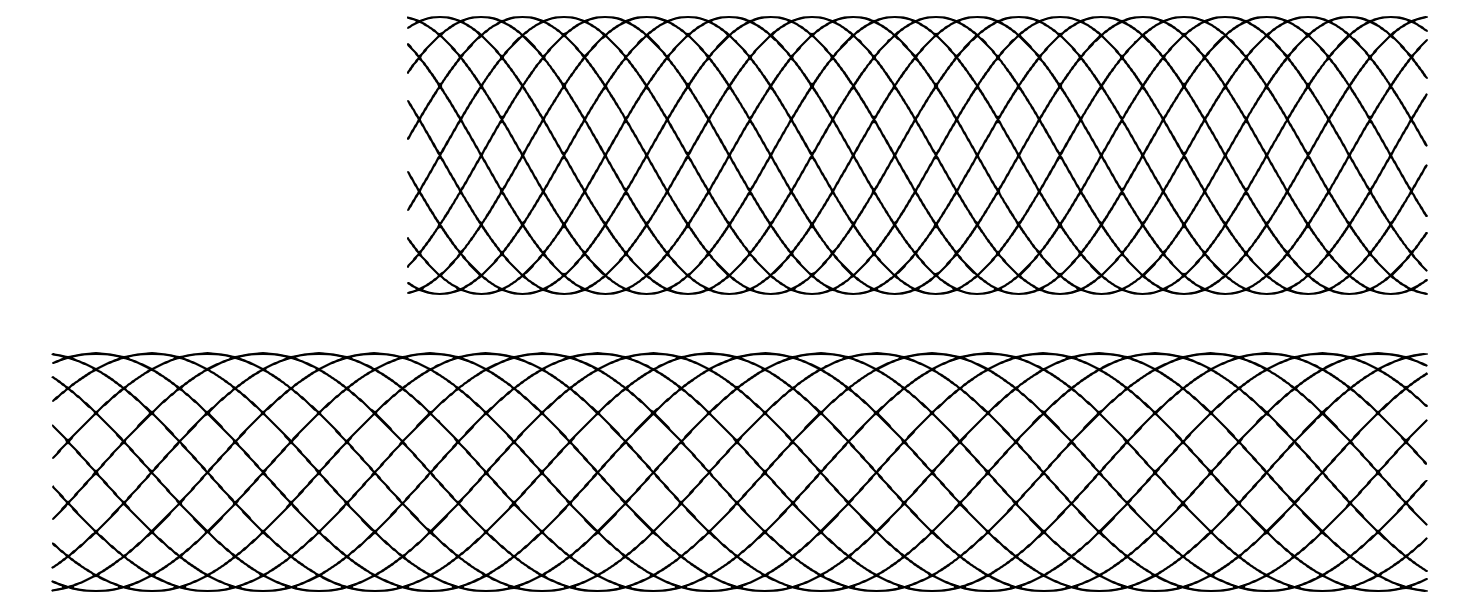
\includegraphics[width=0.9\linewidth]{chapter4/Figures/Stent/Basic_Stents.png}};
%Straight Lines [id:da13251976899948248] 
\draw    (33.48,26.99) -- (33.45,78.98) ;
\draw [shift={(33.45,78.98)}, rotate = 270] [color={rgb, 255:red, 0; green, 0; blue, 0 }  ][line width=0.75]    (0,5.59) -- (0,-5.59);
\draw [shift={(33.48,26.99)}, rotate = 270] [color={rgb, 255:red, 0; green, 0; blue, 0 }  ][line width=0.75]    (0,5.59) -- (0,-5.59);
%Straight Lines [id:da1385922115666558] 
\draw    (33.58,90.68) -- (33.45,135.41) ;
\draw [shift={(33.45,135.41)}, rotate = 270] [color={rgb, 255:red, 0; green, 0; blue, 0 }  ][line width=0.75]    (0,5.59) -- (0,-5.59);
\draw [shift={(33.58,90.68)}, rotate = 270] [color={rgb, 255:red, 0; green, 0; blue, 0 }  ][line width=0.75]    (0,5.59) -- (0,-5.59);
%Straight Lines [id:da1456300945097566] 
\draw    (41,144) -- (291,144) ;
\draw [shift={(291,144)}, rotate = 180] [color={rgb, 255:red, 0; green, 0; blue, 0 }  ][line width=0.75]    (0,5.6) -- (0,-5.6);
\draw [shift={(41,144)}, rotate = 180] [color={rgb, 255:red, 0; green, 0; blue, 0 }  ][line width=0.75]    (0,5.6) -- (0,-5.6);
%Straight Lines [id:da38319342809648804] 
\draw    (106,19) -- (291,19) ;
\draw [shift={(291,19)}, rotate = 180] [color={rgb, 255:red, 0; green, 0; blue, 0 }  ][line width=0.75]    (0,5.6) -- (0,-5.6);
\draw [shift={(106,19)}, rotate = 180] [color={rgb, 255:red, 0; green, 0; blue, 0 }  ][line width=0.75]    (0,5.6) -- (0,-5.6);

% Text Node
\draw (18,48) node [anchor=north west][inner sep=0.75pt]   [align=left] {$\displaystyle r_{1}$};
% Text Node
\draw (18,108) node [anchor=north west][inner sep=0.75pt]   [align=left] {$\displaystyle r_{2}$};
% Text Node
\draw (187,0) node [anchor=north west][inner sep=0.75pt]   [align=left] {$\displaystyle L_{1}$};
% Text Node
\draw (160,148) node [anchor=north west][inner sep=0.75pt]   [align=left] {$\displaystyle L_{2}$};


\end{tikzpicture}
